\subsection{Métricas de evaluación}

La evaluación cuantitativa del desempeño de sistemas de clasificación y calibración requiere métricas que capturen la calidad predictiva del modelo. Resulta fundamental seleccionar métricas apropiadas que reflejen los objetivos operativos del sistema.

\subsubsection{Métricas para clasificación}

La matriz de confusión constituye la representación fundamental del desempeño de un clasificador, tabulando predicciones versus etiquetas verdaderas. Para un problema de $C$ clases, la matriz de confusión $\mathbf{M} \in \mathbb{R}^{C \times C}$ tiene elementos:

\begin{equation}
M_{ij} = \sum_{k=1}^{N} \mathbb{1}[y_k = i \land \hat{y}_k = j]
\end{equation}

donde $y_k$ es la clase verdadera de la muestra $k$, $\hat{y}_k$ es la clase predicha, y $\mathbb{1}[\cdot]$ es la función indicadora. Los elementos diagonales representan clasificaciones correctas, mientras que los elementos fuera de la diagonal representan errores.

\begin{table}[h]
\centering
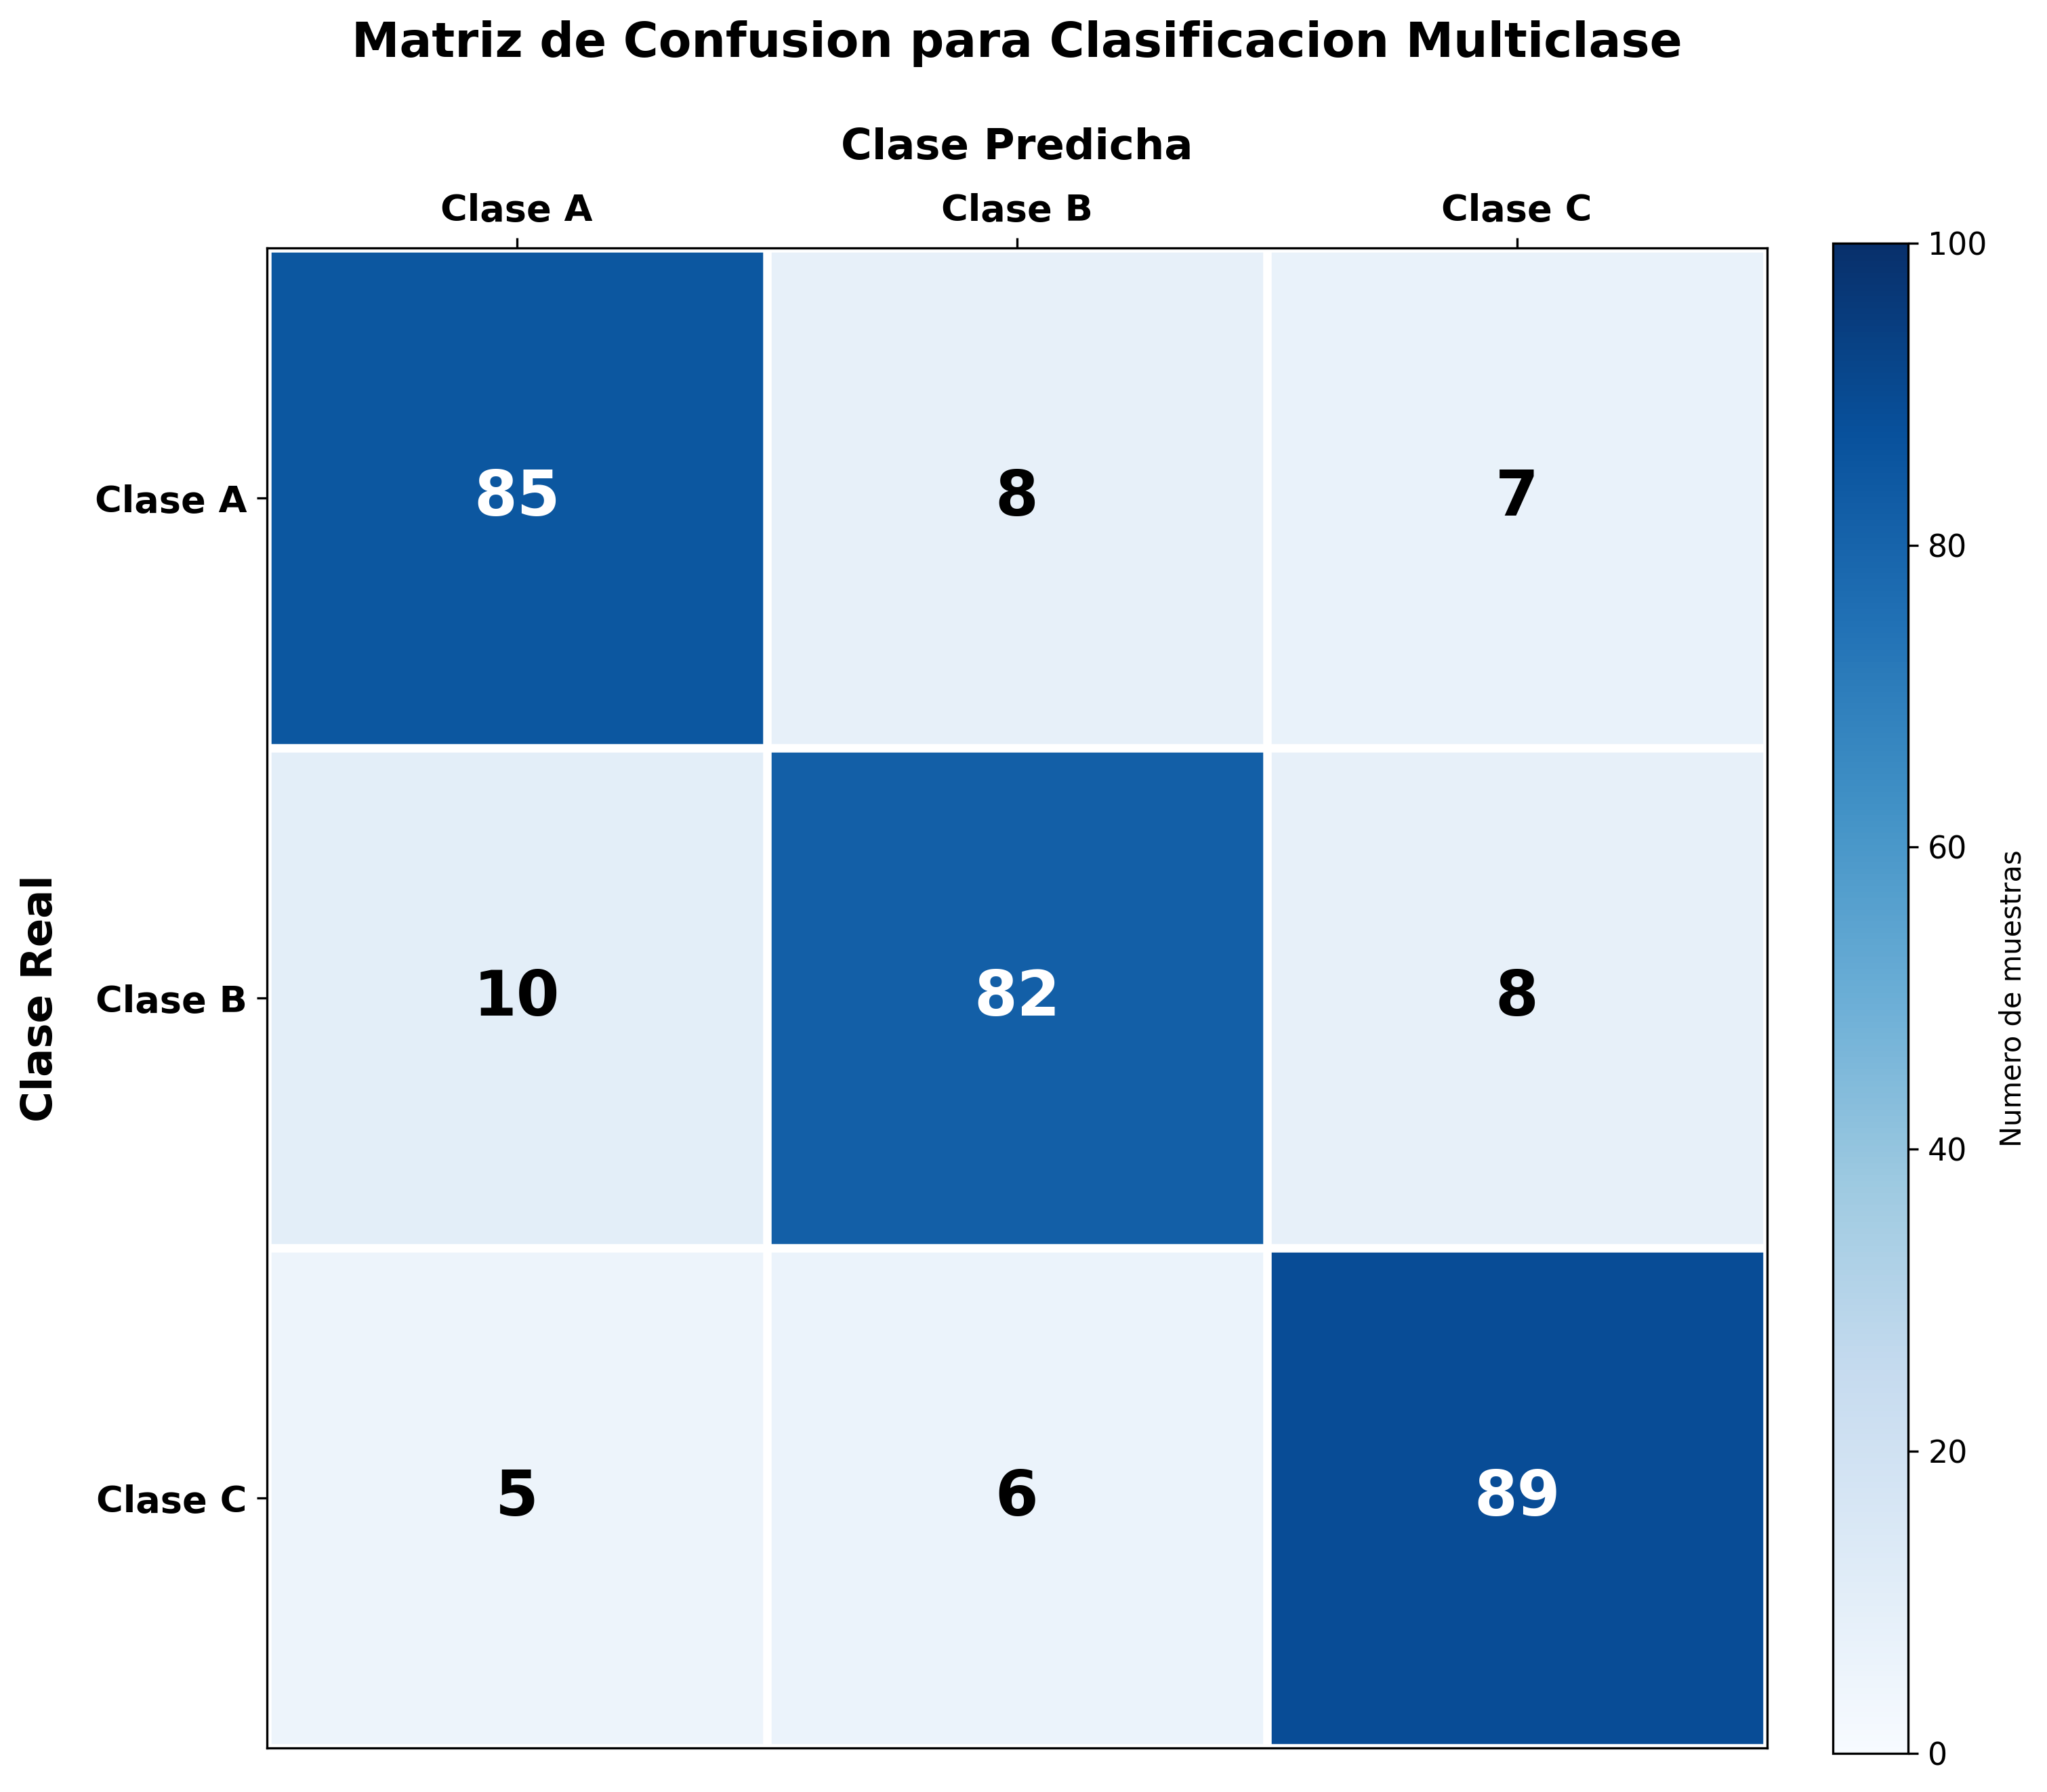
\includegraphics[width=0.65\textwidth]{imagenes/matriz_confusion_ejemplo.png}
\caption{\textit{Matriz de confusión de referencia para clasificación multiclase}}
\label{fig:matriz_confusion}
\end{table}

La precisión cuantifica la proporción de predicciones positivas correctas: $\text{Precision} = \text{TP}/(\text{TP} + \text{FP})$. La exhaustividad mide la proporción de casos positivos reales identificados: $\text{Recall} = \text{TP}/(\text{TP} + \text{FN})$. Existe un compromiso inherente entre precisión y recall: aumentar el umbral de decisión incrementa la precisión pero reduce el recall, y viceversa.

\subsubsection{Métricas para calibración espacial}

En sistemas de calibración píxel-milímetro, se emplean métricas de error continuo. El error cuadrático medio (RMSE) cuantifica la magnitud típica de los errores:

\begin{equation}
\text{RMSE} = \sqrt{\frac{1}{N}\sum_{i=1}^{N}(y_i - \hat{y}_i)^2}
\end{equation}

El coeficiente de determinación $R^2$ mide la proporción de varianza explicada por el modelo:

\begin{equation}
R^2 = 1 - \frac{\sum_{i=1}^{N}(y_i - \hat{y}_i)^2}{\sum_{i=1}^{N}(y_i - \bar{y})^2}
\end{equation}

Valores de $R^2$ cercanos a 1 indican excelente ajuste lineal del modelo. Para aplicaciones de agricultura de precisión, se requiere bajo RMSE (típicamente <2mm) y alto $R^2$ (>0.99) para garantizar precisión en el posicionamiento.
